\begin{center}
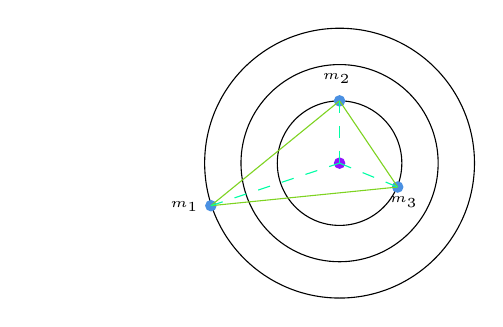
\begin{tikzpicture}[x=0.75pt,y=0.75pt,yscale=-1,xscale=1]
%uncomment if require: \path (0,300); %set diagram left start at 0, and has height of 300

%Straight Lines [id:da7411767697224816] 
\draw    (100,102) ;
%Shape: Circle [id:dp9490684003061072] 
\draw   (220,140) .. controls (220,123.43) and (233.43,110) .. (250,110) .. controls (266.57,110) and (280,123.43) .. (280,140) .. controls (280,156.57) and (266.57,170) .. (250,170) .. controls (233.43,170) and (220,156.57) .. (220,140) -- cycle ;
%Shape: Circle [id:dp9814343956363334] 
\draw   (202.5,140) .. controls (202.5,113.77) and (223.77,92.5) .. (250,92.5) .. controls (276.23,92.5) and (297.5,113.77) .. (297.5,140) .. controls (297.5,166.23) and (276.23,187.5) .. (250,187.5) .. controls (223.77,187.5) and (202.5,166.23) .. (202.5,140) -- cycle ;
%Shape: Circle [id:dp685701971148887] 
\draw   (185,140) .. controls (185,104.1) and (214.1,75) .. (250,75) .. controls (285.9,75) and (315,104.1) .. (315,140) .. controls (315,175.9) and (285.9,205) .. (250,205) .. controls (214.1,205) and (185,175.9) .. (185,140) -- cycle ;
%Shape: Circle [id:dp08570959225680785] 
\draw  [color={rgb, 255:red, 144; green, 19; blue, 254 }  ,draw opacity=1 ][fill={rgb, 255:red, 144; green, 19; blue, 254 }  ,fill opacity=1 ] (252.5,140) .. controls (252.5,138.62) and (251.38,137.5) .. (250,137.5) .. controls (248.62,137.5) and (247.5,138.62) .. (247.5,140) .. controls (247.5,141.38) and (248.62,142.5) .. (250,142.5) .. controls (251.38,142.5) and (252.5,141.38) .. (252.5,140) -- cycle ;
%Shape: Circle [id:dp47337912414359584] 
\draw  [color={rgb, 255:red, 74; green, 144; blue, 226 }  ,draw opacity=1 ][fill={rgb, 255:red, 74; green, 144; blue, 226 }  ,fill opacity=1 ] (280.5,151.5) .. controls (280.5,150.12) and (279.38,149) .. (278,149) .. controls (276.62,149) and (275.5,150.12) .. (275.5,151.5) .. controls (275.5,152.88) and (276.62,154) .. (278,154) .. controls (279.38,154) and (280.5,152.88) .. (280.5,151.5) -- cycle ;
%Shape: Circle [id:dp40050388744279153] 
\draw  [color={rgb, 255:red, 74; green, 144; blue, 226 }  ,draw opacity=1 ][fill={rgb, 255:red, 74; green, 144; blue, 226 }  ,fill opacity=1 ] (252.5,110) .. controls (252.5,108.62) and (251.38,107.5) .. (250,107.5) .. controls (248.62,107.5) and (247.5,108.62) .. (247.5,110) .. controls (247.5,111.38) and (248.62,112.5) .. (250,112.5) .. controls (251.38,112.5) and (252.5,111.38) .. (252.5,110) -- cycle ;
%Shape: Circle [id:dp5599587744609031] 
\draw  [color={rgb, 255:red, 74; green, 144; blue, 226 }  ,draw opacity=1 ][fill={rgb, 255:red, 74; green, 144; blue, 226 }  ,fill opacity=1 ] (190.5,160.5) .. controls (190.5,159.12) and (189.38,158) .. (188,158) .. controls (186.62,158) and (185.5,159.12) .. (185.5,160.5) .. controls (185.5,161.88) and (186.62,163) .. (188,163) .. controls (189.38,163) and (190.5,161.88) .. (190.5,160.5) -- cycle ;
%Straight Lines [id:da384151252822579] 
\draw [color={rgb, 255:red, 126; green, 211; blue, 33 }  ,draw opacity=1 ]   (188,160.5) -- (278,151.5) ;
%Straight Lines [id:da24848451118665693] 
\draw [color={rgb, 255:red, 126; green, 211; blue, 33 }  ,draw opacity=1 ]   (188,160.5) -- (250,110) ;
%Straight Lines [id:da8234484439529937] 
\draw [color={rgb, 255:red, 126; green, 211; blue, 33 }  ,draw opacity=1 ]   (250,110) -- (278,151.5) ;
%Straight Lines [id:da4853630824410369] 
\draw [color={rgb, 255:red, 0; green, 255; blue, 165 }  ,draw opacity=1 ] [dash pattern={on 4.5pt off 4.5pt}]  (188,160.5) -- (250,140) ;
%Straight Lines [id:da04897594598262511] 
\draw [color={rgb, 255:red, 0; green, 255; blue, 165 }  ,draw opacity=1 ] [dash pattern={on 4.5pt off 4.5pt}]  (250,140) -- (278,151.5) ;
%Straight Lines [id:da013808732174074745] 
\draw [color={rgb, 255:red, 0; green, 255; blue, 165 }  ,draw opacity=1 ] [dash pattern={on 4.5pt off 4.5pt}]  (250,110) -- (250,140) ;

% Text Node
\draw (167.33,157) node [anchor=north west][inner sep=0.75pt]  [font=\tiny] [align=left] {$\displaystyle m_{1}$};
% Text Node
\draw (240.67,95.33) node [anchor=north west][inner sep=0.75pt]  [font=\tiny] [align=left] {$ $$\displaystyle m_{2}$};
% Text Node
\draw (273,155) node [anchor=north west][inner sep=0.75pt]  [font=\tiny] [align=left] {$\displaystyle m_{3}$};


\end{tikzpicture}

\end{center}
